%\documentstyle[emulateapj,apjfonts,epsfig]{article}
\documentclass{emulateapj}
\usepackage{amsmath, mathtools}

%\documentclass[12pt,preprint]{aastex}
%\usepackage{emulateapj5,apjfonts}

\newcommand{\EXO}{\mbox{EXO 0748-676}}
\newcommand{\keV}{${\rm keV}$}
\newcommand{\Fe}{${\rm Fe} \ $}
\newcommand{\Mn}{${\rm Mn} \ $}
\newcommand{\Cr}{${\rm Cr} \ $}
\newcommand{\V}{${\rm V} \ $}
\newcommand{\Ti}{${\rm Ti} \ $}
\newcommand{\Sc}{${\rm Sc} \ $}
\newcommand{\Ca}{${\rm Ca} \ $}
\newcommand{\be}{\begin{equation}}
\newcommand{\ee}{\end{equation}}
\newcommand       \etaeff       {\eta}
\newcommand       \tff          {\tau_{\rm ff}}
\newcommand       \tdyn         {\tau_{\rm dyn}}


\shorttitle{Neutron Star Redshift Measurements} 
\shortauthors{Bildsten, Chang and Paerels}

\begin{document}

\title{NEED TITLE}

\author{some people}


                        %%%%%%%%%%%%%%%%%%%%%%%%
                        %       abstract       %
                        %%%%%%%%%%%%%%%%%%%%%%%%
\begin{abstract}

write this

\end{abstract}

\keywords{diffusion -- nuclear reactions -- 
stars: abundances, surface -- stars: neutron -- X-rays: binaries, bursts}

\section{Introduction}

The rapid formation of stars remains an unsolved problem in astrophysics.

Here we will focus on the physics of rapid star formation and accretion.  An early model of Shu (1977) estimated the accretion rate onto stars by 
assuming that stars form from hydrostatic cores
supported by thermal gas pressure. The accretion
rate in his model was independent of time, given
by $M = m_0c_s^3/G$, where $c_s$  is the
sound speed in molecular gas, and $m_0 = 0.975$.
Shu (1977) predicted a maximum accretion rate was $yr^{-1}$, which is too small to explain
the origin of massive stars.

Later workers overcame the difficulty with the accretion rate by adopting the turbulence speed in lieu of the sound speed (Myers \& Fuller 1992, McLaughlin \& Pudritz 1997, McKee \& Tan 2003). In doing so they were able to replace the slower signal speed of sound with the faster turbulent speed.  However, they rely on assuming that a hydrostatic core supported by turbulent pressure is the initial condition and that turbulence is static and unaffected by the collapse.  

Recently Murray \& Chang (2015), hereafter MC15, developed a 1-D model of spherical collapse that treat turbulence as a dynamical variable and does not assume that the initial condition is a hydrostatically supported region.  They were able to accomplished this by taking advantage of the recent results of Robertson \& Goldreich (2012) on compressible turbulence. In particular 

{\bf need equation}

Hence, this allowed MC15 to include an energy equation for the turbulent velocity that alongside the equations for mass continuity and momentum gives a set of equations that can be solved in spherical symmetry numerically.  In addition, they were able to analytically show that the results of their calculations gave density and velocity profiles that appear to be in line with both recent numerical calculations (Lee et al 2015) and observations.    

In particular, their basic results are that the run of density asymptotes to 
\be
\rho(r,t)=
\begin{dcases}
\rho(r_0)\left({r\over r_0}\right)^{-3/2}, & r<r_*\\
\rho(R,t)\left({r\over R}\right)^{-k_\rho}, \ k_\rho\approx1.6-1.8 & r>r_*.
\end{dcases}
\ee
Since $k_\rho$ is fairly close to $1.5$ at all radii, taking $r_0=R$
is a fair approximation. 
The infall velocity 
%
\be
u_r(r,t)=
\begin{dcases}
-\Gamma\sqrt{GM_*(t)\over r}, \sim r^{-1/2} & r<r_*\\
-\Gamma\sqrt{GM(r,t)\over r} \sim r^{0.2} & r>r_*,
\end{dcases}
\ee
%
where $\Gamma \approx 0.7$ at small radii, and $\Gamma\approx 1.0$ at
large radii. 

The turbulent velocity 
%
\be
v_T(r,t)=
\begin{dcases}
{1\over 2\etaeff}\Gamma\sqrt{GM_*(t)\over r}, \sim r^{-1/2} & r<r_*\\
{1.2\over \etaeff}\Gamma\sqrt{GM(r,t)\over r} \sim r^{0.2} & r>r_*,
\end{dcases}
\ee
%

The stellar mass increases quadratically with time
%
\be  %$
M_*(t)=\phi M_{\rm cl}\left({t-t_*\over \tff}\right)^2.
\ee  %$
%

The mass accretion rate 
%
\be
\dot M(r,t)=
\begin{dcases}
4\pi R^2\rho(R)u_r(r,t), \sim t\,r^{0} & r<r_*\\
4\pi R^2\rho(R)u_r(r,t) \sim t^0\,r^{0.2} & r>r_*.
\end{dcases}
\ee
%

These results compared favorable with the results of numerical simulations (Lee et al. 2015).  However, it is unclear if the results of 

\section{Detailed Simulations of Turbulent Collapse} \label{sec:simulation setup}

We use the adaptive mesh refinement code FLASH ver. 4.0.1 (Fryxell et al. 
2000
; Dubey
et al.
2008
) to model isothermal, self-gravitating, hydrodynamic turbulence on isothermal gas with three-dimensional (3D),
periodic grids and 8 levels of refinement on a root grid of $128^3$, giving an effective resolution of $32K^3$.  
Self-gravity is computed with a multi-grid Poisson solver (see Ricker 2008), coupled with a fast-Fourier transform solution on the root grid. Similar to (Lee et. al Feb. 2015) our FLASH runs use the Harten-Lax-van Leer-Contact Riemann solver and an unsplit solver. (Lee \& Deane (2009)

We start with a box with the physical length set to $L = 16$pc using periodic boundary condtions. The intial mass density is $\rho = 3x10^{-22}$ and the isothermal, ambient gas is set to a sound speed of $c_s = 2.64x10^{4}$. To initialize our simulations, we drive turbulence by applying a large scale ($1 \le kL \le 2$) solenoidal acceleration field as a momentum and energy source term. We apply this field in the absence of gravity and sink particle formation for 3 dynamical times until a statistical steady state is reached.
{\bf WHY JUST SOLENOIDAL}

This fully developed turbulent state is the initial condition to which we add self-gravity and sink particle formation for our star formation experiments. Sink particles are formed as described in Lee et al. (2014) and described briefly below.  

The gravitational force is computed differently between sink particles than between sink particles and the gas. Sink particle-sink particle forces are computed via direct N-body calculation. While sink particle-gas and gas-sink particle is computed via the multi-grid Poisson solver. As a result of these additional computations, two large scale gravity solutions must be found per timestep as oppose to one. This allows to avoid the computationally expensive task of computing gas-sink particle forces via direct summation.

We have also implemented a new algorithm for mesh refinement in these simulations. As gas collapse under self gravity, certain regions rapidly increase in density. These regions are refined when the Truelove criterion ($\lambda \le 4 \Delta x$) is met. This corresponds to a condition on the density 
\be
\frac{\rho}{\rho_{0}} = 45 \cdot 4^{l} \left( \frac{N_{root}}{128} \right)^2 \left( \frac{16 \text{pc}}{L} \right)^2 \left( \frac{c_{s}}{2.65\text{x}10^4 \text{cm s$^{-1}$}} \right)^2 \left( \frac{3 \text{x}10^{-22} \text{g cm$^{-3}$}}{\rho_{0}} \right)
\label{eq:refinement_criteria}
\ee
 where $l$ is the refinement level, with $l = 0$ corresponding to the root grid. When this density condition is met the local grid is refined by a factor of 2 provided that the maximum refinement level has not reached. 
We reach a maximum of $\rho / \rho_{0} \approx 3 \text{x} 10^{7}$ at $l$ = 8, the maximum refinement level. Thus we traverse nearly 8 orders of magnitude in the density in our AMR simulations.
When the Truelove criterion is met at the highest refinement level, the excess mass in a cell is transferred either to a newly created sink particle or to a sink particle whose accretion radius includes the cell. This behavior is the same as in Lee et al. (2014), albeit at a much higher resolution. We should also note that like Lee et al. (2014), our sink particle creation prescription is different from the prescription of Federrath et al (???) where additional checks need to be performed.
Our base grid's resolution of $128^3$ gives a cell length of $1.2 \text{x} 10^{-1}$pc which is sufficient to resolve the Jean's length
\be
\lambda_J \equiv \sqrt{\frac{\pi c_{s}^2}{G \bar{\rho}}} \approx 3.5 \text{pc}
\ee


\section{Numerical Results}

To initialize our simulation, we begin by applying solenoidal stirring forces to the uniform, periodic simulation volume at the root grid resolution of $128^3$ until statistical equilibrium is reached (approximately three crossing times). After this equilibrium is established, we then apply self gravity, adaptive mesh refinement, and sink particle creation. In Figure \ref{fig:entire projection} we show a projection along the z-axis of the entire simulation volume that has up to 8 levels of refinement, giving an effective resolution of $32\,{\rm K}^3$. Regions that are highly refined are the densest regions which are smoother than the low-density more pixelated regions.
\begin{figure}
\plotone{movieframe_quad2_0498.png}
\caption{Projection of the density along the z-axis of the entire simulation volume. The root grid is $128^3$ with up to 8 levels of refinement, giving an effective resolution of $32\,{\rm K}^3$. This snapshot is taken $2.8$Myr after star formation is turned on. \label{fig:entire projection}}
\end{figure}

The high density regions appear to be organized along filaments. These filaments span most of the simulation size, and have a width of 0.5 to 1 pc. Moreover, these filaments appear to flow into large clumps. This is in line with previous work including Lee et al. 2014. These clumpy regions have the highest densities and, hence, are prone to fulfill the criterion for star particle formation.  

At the instance in time shown in Figure \ref{fig:entire projection}, a total of 20 {\bf GET ACCURATE COUNT} star particles have been formed. A couple of these star particles are formed in isolation though the majority formed in binaries and there is a ring of ten in one region. They congregated in several star forming regions shown in Figure \ref{fig:star forming regions}. In these regions, the sink particles that are formed lay within 0.1 pc of one another, which reflects that the highest density regions are concentrated toward the center. Visually, the character of accretion at the this outer scale appear to flow along filaments, though previous work (Lee et al. 2014) has shown that the majority of accretion is spherical. We discuss this more quantitatively below {\bf INCLUDE A STUDY OF LARGE SCALE ACCRETION}


\begin{figure*}
\plottwo{Disk_0132_0000.png}{movie_quad3_frame_0320_part_0000_05pc.png}
\caption{Cut of the two star forming regions. The region on the right formed a single isolated particle, after two filaments {\bf INCLUDE5PC image? } had collided.\label{fig:star forming regions}}
\end{figure*}

% Start with quad3 gold standard

The first particle formed in isolation and remained isolated for the remainder of the simulation run. It is $\approx 1.6x10^5\text{yrs}$ old and is $\approx 10 M_{\odot}$ 

%% Include image of the velocity and disk






The first family of three star particles is shown in Figure \ref{fig:snapshots} and the second family of two star particles is shown in Figure \ref{fig:snapshots 2}.  We plot these particles and their surrounding $4\times 10^{-2}$ pc region as slices perpendicular to the local angular momentum vector.  We determine the local angular momentum vector by taking a $0.01$ pc region about the star particle to calculate the angular momentum vector.  It is clear from these plots that the clumpy filamentary nature of the local star forming environment extends down to much smaller scales than we have been able to probe in previous work (Lee et al. 2014).  

At small radii (similar to $10^{-2}$ pc), a protostellar disk appears in all five snapshots. The radial size of these disks varies. These disks also show a coherent sense of rotation about a common axis, e.g., no counter-rotating disks. In addition, some of the snapshots show multiple high density regions. This could be a result of accretion of high density clumps or fragmentation in the disk or streams.  

We also include a zoom-out picture of the same region, which is the same for all three stars (lower right plot in Figure \ref{fig:snapshots}, bottom plot in Figure \ref{fig:snapshots 2}).  While this is not unexpected as star formation is clustered, the large scale dynamics are determined by the larger region.  We should note that these star particles are within about 0.1 pc of each other in their respective families.  

%\begin{figure*}
%\plottwo{movie_disk_0132_0001.png}{movie_disk_0132_0003.png}
%\plottwo{movie_disk_0132_0000.png}{Disk_0132_0000.png}
%\caption{The upper frames, and the bottom left frame show slices along the angular momentum axis of three local particles in one of the regions demonstrating significant star formation.  Each of the zoomed-in slices have a radius of $0.02$ pc.  To determine the angular momentum axis, we take a $0.01$ pc region about the densest local point and calculate the angular momentum vector.  We then take a slice in the plane normal to the angular momentum vector to plot the regions around these dense points.  The bottom right frame shows the zoomed-out region of formation, with a radius of $1.5$ pc.    \label{fig:snapshots}}
%\end{figure*}


\begin{figure*}
\plottwo{movie_disk_0132_0001.png}{movie_disk_0132_0003.png}
\plottwo{movie_disk_0132_0000.png}{Disk_0132_0000.png}
\caption{The upper frames, and the bottom left frame show slices along the angular momentum axis of three local particles in one of the regions demonstrating significant star formation.  Each of the zoomed-in slices have a radius of $0.02$ pc.  To determine the angular momentum axis, we take a $0.01$ pc region about the densest local point and calculate the angular momentum vector.  We then take a slice in the plane normal to the angular momentum vector to plot the regions around these dense points.  The bottom right frame shows the zoomed-out region of formation, with a radius of $1.5$ pc.    \label{fig:snapshots}}
\end{figure*}

\begin{figure*}
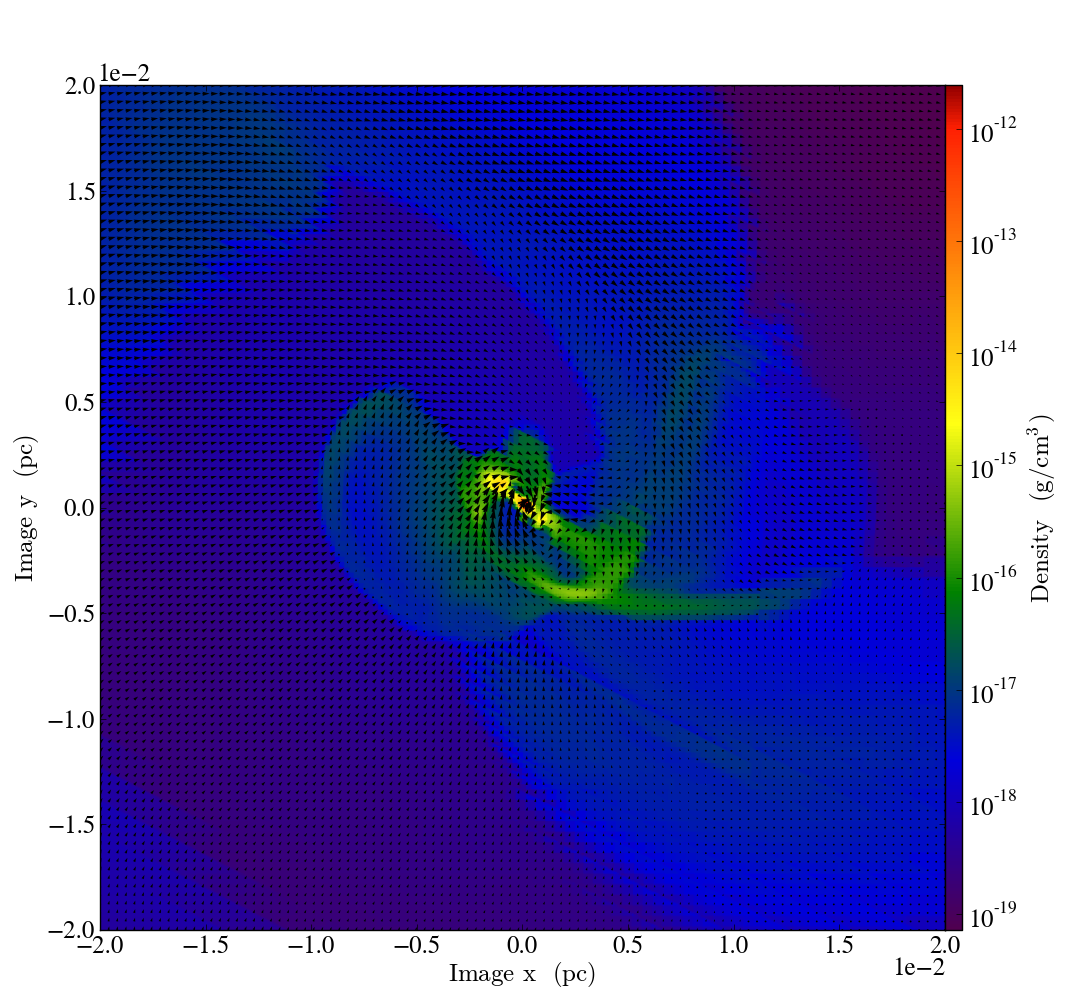
\includegraphics[width=0.48\textwidth]{movie_disk_0132_0002.png}
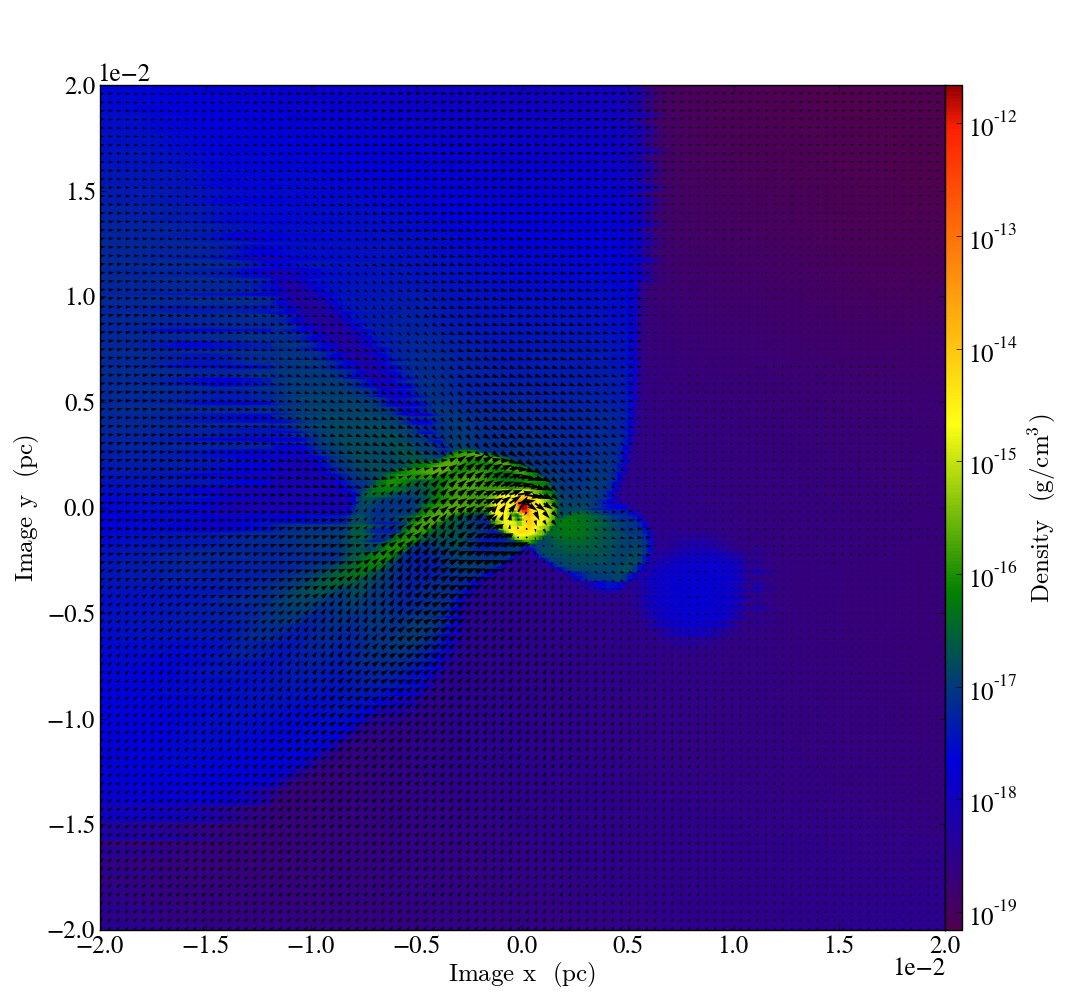
\includegraphics[width=0.48\textwidth]{movie_disk_0132_0004.png}
\centering{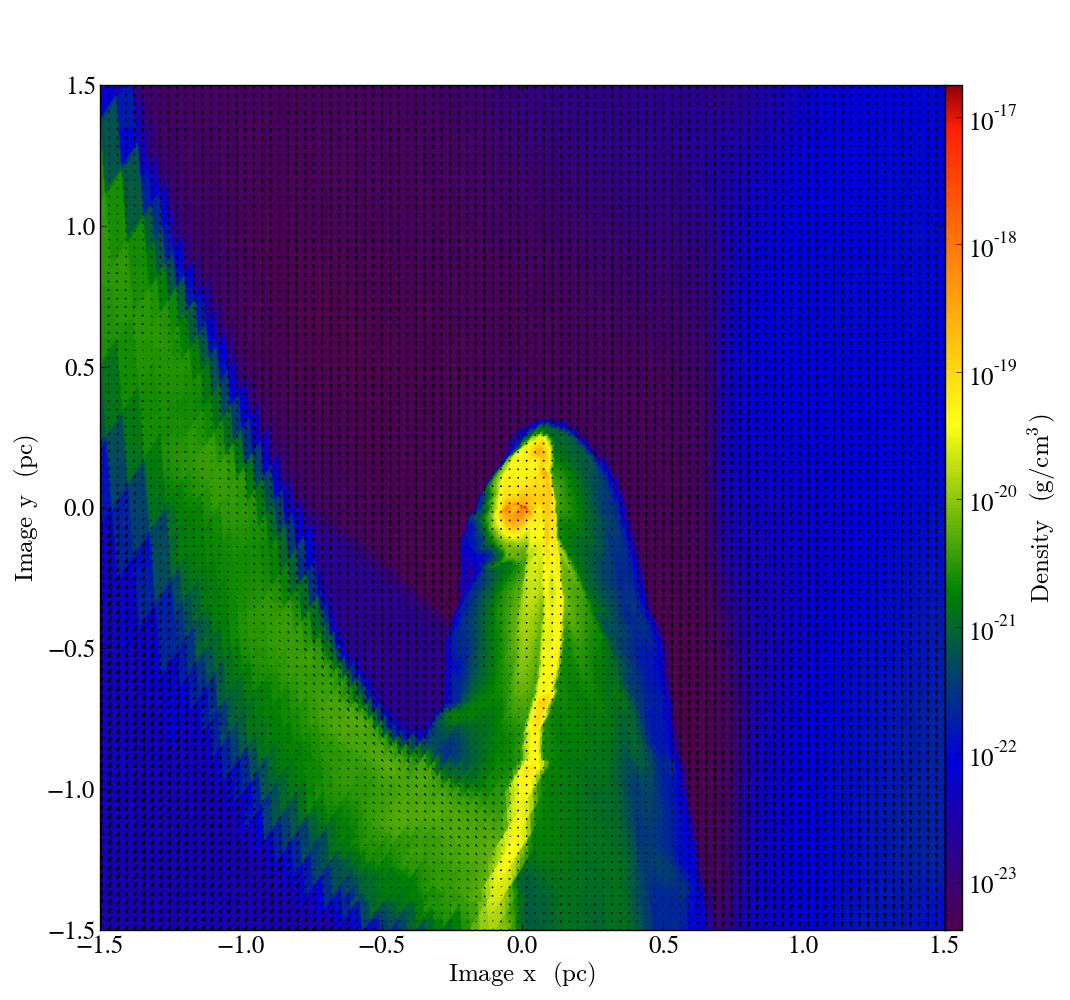
\includegraphics[width=0.48\textwidth]{Disk_0132_0002.png}}
\caption{The upper frames show the zoomed-in slices along the angular momentum axis of the local particles in the second region of significant star production.  Again, each of the zoomed-in slices have a radius of $0.02$ pc.  The bottom frame shows the zoomed out region, with a radius of $1.5$ pc.  \label{fig:snapshots 2}}
\end{figure*}

{\bf ARE THESE DISK GRAVITATIONALLY STABLE?}


\begin{figure*}
\plottwo{Average_5_013.pdf}{Average_5_24.pdf}
\plottwo{Average_02_013.pdf}{Average_02_24.pdf}
\caption{Here we show the mass accretion rates as a function of density.  The upper figures are displaying rates corresponding to a region of $0.5$ pc around the particle, while the lower figures are showing a radius of $0.02$ pc.  The two plots on the left show the region with three particles forming, and the plots on the right show the region with two particles forming.  The more massive region with three particles indicates the mass is coming in at a density value roughly three times the average density, and the curves are similar between the smaller and larger radii.  The graph for the less massive region on the right shows a distinctly separate profile between the larger and the smaller radius.   \label{fig:accretion average rho}}
\end{figure*}

In prior work, we examined the geometry of accretion, i.e., does the accretion proceed along filament or over 4$\pi$ steradian, by plotting the cumulative accretion rate as a function of density. In Figure \ref{fig:accretion average rho}, we plot the cumulative accretion rate as a function of density, normalized to the average density in shells of radii 0.5 (upper plots) and 0.02 pc (lower plots).  Plots on the left are associated with the more massive star forming region, where 3 star particles reside and plots on the right are associated with the less massive star forming region, where two star particles reside.  The density where 50\% of the accretion is accounted for occurs at $\rho/\bar{\rho} \approx 3$ for the more massive star forming region and appears to be independent of whether the shell has a radius of 0.5 or 0.02 pc.  This suggests that the accretion is proceeding along filaments.  Similarly, the less massive star forming region has half of the accretion account for at $\rho/\bar{\rho} \approx 10$ at r=0.5 pc, again suggesting filamentary accretion.  However, this filamentary nature of accretion does not maintain itself to lower radii, where at 0.02 pc, the 50\% point in cumulatiove accertion occurs at $\rho/\bar{\rho} \approx 1$, which suggest accretion is spherical.

Figures \ref{fig:geometry} and \ref{fig:geometry 2} show the moments of inertia for the three star particles in the more massive and less massive star forming regions, respectively.  For the more massive star forming region (Fig. \ref{fig:geometry}), note that the moments of inertia are identical for radii greater than $2e-2$, due the fact that these three star particles sit in the same massive star forming region. This is similarly true for the less massive region for $r\gtrsim 0.1$ pc.  At small radii, the distribution of gas appears to be flattened or rod-like, which is implied by the relative values of the three principle axes.  Around $r\approx 0.02$ and $r \approx 0.1$ pc, respectively, the geometry of the gas is relatively spherical.  Outside this region, the gas become flatter again. However, the flattened distributions seen at small and larger radii may also reflect the effect of streams of gas or gravitational instabilities that are associated with the accretion. 

\begin{figure}
\plotone{geometry_4_cum.pdf}
\caption{Plots of the moments of inertia for the three star particles in the more massive star forming region.  Note that the moments of inertia are identical for radii greater than $2e-2$, due the fact that these three star particles sit in the same massive star forming region.  Inside this region, we find that the two largest moments of inertia are close in value to each other, suggesting that the geometry of the gas resembles a flattened distribution. Around $r\approx 0.02$ pc, the geometry of the gas becomes relatively spherical.  Outside this region, the gas become flatter again. However, the flattened distributions seen at small and larger radii may also reflect the effect of streams of gas that might drive the accretion. 
\label{fig:geometry}}
\end{figure}

\begin{figure}
\plotone{geometry_4_cum.pdf}
\caption{$Geometry_2$ and $geometry_4$ Plots of the moments of inertia for the two star particles in the less massive star forming region.  The moments of inertia for these particles are identical down to a radius of $r\approx 0.1$ pc
\label{fig:geometry 2}}
\end{figure}


\subsection{Radial Profile of Velocity after Star Formation}

These simulations display much more complicated dynamics than is captured by the simple analytic theory of Murray and Chang 2014.  In spite of this, we proceed to compare radially averaged profiles around these high density points to their analytic theory.  Toward this end, we construct radial profiles around the most massive star particle in each of the star forming regions.

{\bf Include condition to place in which shell?}
We start with the isolated case seen in the right image of figure \ref{fig:star forming regions}. In Figure \ref{fig:quad3_320_velocity}, we show the radial distribution of the radial infall velocity $\vec{v}_r$, the angular velocity $\vec{v}_{\phi}$, the keplerian velocity $\vec{v}_{K}$ and the turbulent velocity $\vec{v}_{t}$ in spherical shells around the star particle. In calculating these values, we use a spherical geometry, though we're working on subtracting the velocity in a  cylindrical geometrical case as well. 
FLASH provides us with $\vec{v}$ in each cell, which includes the bulk flow of the cloud. To remove the bulk flow velocity we calculate the momentum of the material inside of (including) the thin spherical shell we're interested in. We then remove that mass weighted velocity from the total velocity. This give us our total velocity line in figure \ref{fig:quad3_320_velocity} (the magenta "dot" line). 
To obtain the radial infall velocity (blue triangle line) we use $p_r[i] = \vec{v}_r[i] \cdot \vec{r}[i] * m[i]$ to obtain the radial momentum of the ith cell inside the spherical shell of interest. We then sum over all $p_{r}[i]$ that are in the shell, divide by the total mass in the shell and obtain the mass weighted radial velocity for that shell. 
To obtain $\vec{v}_{\phi}$ we start with equation \ref{eq:calc v_phi} as we need to know the directionality of $\vec{v}_{\phi}$ in order to properly subtract it to obtain $\vec{v}_{t}$.

\be
\vec{v}_{\phi} = \vec{\Omega} \times \vec{r}
\label{eq:calc v_phi}
\ee
With \ref{eq:calc v_phi} in mind, we start with what we know from FLASH, $\vec{r}$ and $\vec{v}$ for each cell, and use that to obtain $\vec{L}$

\be
\vec{L}_{shell} = \sum{\vec{r} \times \vec{v} * m}
\label{eq:calc L shell}
\ee
where the sum is over all cells in the shell and $\vec{L_{shell}}$ is the angular momentum vector of the shell. We also calculate the elements of the moment of Inertia tensor for each cell.

\be
I_{ii} = (x_{jj}^2 + x_{kk}^2) * m[n]
I_{ij} = -x_{i}[n]*x_{j}[n] * m[n]
\label{eq:moment of inertia}
\ee
for the nth cell in the shell. We sum over all cells in the shell to obtain the Inertia tensor for each shell.
We use $\vec{L}$ and $I$ to obtain $\Omega$

\be
I^{-1}\vec{L} = \Omega
\label{eq:Obtain Omega}
\ee
having obtained $\Omega$ we refer back to \ref{eq:calc v_phi} and plot the results in figure \ref{fig:quad3_320_velocity} where the black +'s are $v_{\phi}$.

In calculating the turbulent velocity we used a slightly more intelligent approach then the brute force subtract in quadrature.
\be
\vec{v}_{t} = \sqrt{\vec{v}^2 + \vec{v}_{\phi}^2 + \vec{v}_{r}^2 - 2(\vec{v} \cdot \vec{v}_{\phi}) - 2(\vec{v} \cdot \vec{v}_{r}) + 2(\vec{v}_{\phi} \cdot \vec{v}_{r})}
\label{eq:Vrms subtraction}
\ee

as a check that we were accounting for all of the velocity that we started with, we added the velocities in quadrature: $\vec{v}_{sum} = \sqrt{\vec{v}^2 + \vec{v}_{\phi}^2 + \vec{v}_{r}^2 + \vec{v}_{t}}$ and it traces $\vec{v}$ extremely well.

The dashed red line is the Keplerian velocity:
\be
\vec{v}_{K} = \sqrt{G m \over \vec{r}}
\label{eq:Kepler velocity}
\ee

The authors want to touch upon the fact that the total velocity ($\vec{v}$) does not quite match up with $\vec{v}_{K}$. The reason is, as one can see from the plotted line of $c_s$ in figure (\ref{fig:quad3_320_velocity}) the flows are mostly super or trans-sonic. Thus, one should expect to see shocks, which would remove some energy from the flow in the form of thermal heating. These simulations, as mentioned in section \ref{sec:simulation setup} are isothermal. Thus, the heating that results from these shocks is immediately radiated away.

%\begin{equation}
%p_r[i] = \vec{v_r}[i] \cdot \vec{r}[i] * m[i]
%vr_nomass[i] = (vx[i]*x[i] + vy[i]*y[i] + vz[i]*z[i])/r[i]
%vr = vr_nomass[i] * cellMass[i]%
%
%\label{eq:obtain_vr}
%\end{equation}


\begin{figure}
\plotone{velocity_quad3_0320_shellsphere_000.pdf}
\caption{Plot of the run of velocities for the isolated star particle seen in the right image of figure \ref{fig:star forming regions}. The dotted line in magenta is the numerical total velocity. The dot-dash green line is the turbulent velocity, the blue triangle line is the radial infall while the black $+$ is $v_{\phi}$. A color version of this plot is available online.
\label{fig:quad3_320_velocity}}
\end{figure}

\subsection{Radial Profile of Collapse}

These simulations display much more complicated dynamics than is captured by the simple analytic theory of Murray and Chang 2014.  In spite of this, we proceed to compare radially averaged profiles around these high density points to their analytic theory.  Toward this end, we construct radial profiles around the most massive star particle in each of the star forming regions.

In Figure \ref{fig:132 000 graphs}, we show the radial distribution of $\rho$, $v_r$, $v_t$, $M(r)$, $\dot{M}$, and the density distribution function around the three star particles.  In the top left plot, we show a slice of the region perpendicular to the z-axis.  The top right plot shows $\rho(r)$ alongside lines of $r^{-3/2}$, $r^{-2}$ and $r^{-5/2}$.  Here we find that at small radii, $\rho(r)\sim r^{-2}$ at small radii and $\rho(r) \sim r^{-3/2}$ between 0.1 - 1 pc. At other radii, the density profile is surprisingly steep, steeper than even $r^{-5/2}$.

The velocity profiles show similar change in behavior in the transition increasing from small radii, around $r\approx 0.02$ pc.  The radial velocity tends to increase to $0.02$ pc, and then decreases following the slope noted in the red line of 0.5.  This demarcation from the smaller radii to larger is due to the disk-like shape of the star particle at the smaller radii.  The turbulent velocity, green line, decreases inward.  

The middle right graph shows the mass as a function of radius.  The mass monotonically increases.  However there is a flattening around $0.1$ pc before it steepens again.  This is important because this region behaves similarly to a point mass.  Which is also reflected in the density profile and the radial velocity profile where $\rho \sim r^-1.5$ and $v_r \sim r^{-1/2}$ as shown by MC15 around point masses.  

The bottom left graph shows the mass accretion rates for all three particles in the more massive region.  At small radii, the drop off in $\dot M$ is due to the presence of a disk, the drop off at larger radii is due to the step density profile.  

The bottom right graph depicts the density PDF for three different radii.  Here it roughly corresponds to the density profile shown in the top right plot.  For instance, the PDF inside a 1 pc sphere has a slope of $\rho ^-1.3$ which corresponds to a radial profile of $\rho \sim r^-2.5$, whereas for a 2 pc sphere, the slope is now $\rho ^-1.5$ corresponding to radial profile of $\rho \sim r^-2$.  

The comparative plots for the less massive region are shown in \ref{fig:132_002_graphs}.  The upper left graph shows a slice perpendicular to the z axis in the plane of peak density around this region of star formation.  The graph shows a single filamentary strand of accretion towards the inner disk-like structure.  

Here again the top right plot shows $\rho(r)$ alongside lines of $r^{-3/2}$, $r^{-2}$ and $r^{-5/2}$.  Between $0.01\,{\rm pc} \lesssim r \lesssim 0.1$ pc, $\rho$ closely matches the slope of $r^{-3/2}$.  This same region shows a flattening in the mass profile (middle right plot) and a radial velocity profile that is similar to $r^{-1/2}$ (middle left plot).  This region also shows flat $\dot{M}$ profile (lower left plot).  For larger radii, the density profile shows a break toward a steeper power law in $r$ and the velocity profiles shows a switch to rising with $r$ rather than falling with $r$.  The mass profile shows a continued monotonic increase with $r$, indicating that the mass is dominated by the gas and not by a central mass.  

In addition, a sharp spike in density appears at $r = 6e-3$ pc that is notable in the velocity, mass, and $\dot M$, plots as well.  The plot of moments of inertia also indicate that this point is where the two particles begin to diverge most significantly. 

The middle left plot shows the velocity profiles, which also indicate an anomoly at $r \eqsim 6e-3$ pc.  However, the general trend of both turbulent and radial velocity is increasing inward from $r \eqsim 0.1$ pc, and also increasing outward from $r \eqsim 0.1$ pc.

The mass distribution, the middle right plot, again increases monotonically.  The flattening in this less massive region occurs at the notable radius of $r \eqsim 6e-3$ pc, before steepening again.           


%In the left panel of Figure \ref{fig:good_rho_example}, we show the radial density profile around one such high density point. As this figure shows, the radial density profile follows a $r^{-3/2}$ power law in agreement with analytic expections.  This power-law breaks down at small radii, but this is not unexpected as this radii corresponds to the presents of a rotationally support disk.  Such good agreement is not universal for all high density points as shown in the right panel of Figure \ref{fig:bad_rho_example}.  Here the radial density profile follows a $r^{-2}$ power law.  
%\begin{figure*}
%\plottwo{Track_0256_000_rho.png}{Track_0132_000_rho.png}
%\caption{Density as a function of radial position from maximum density point.  The density reaches a maximum of $10^6$ times mean density at $r \approx 10^{-3}$ pc and declines to approximately mean density at $r\approx 3$ pc.  The three straight solid lines are $r^{-3/2}$, $r^{-2}$, and $r^{-5/2}$ power laws. \label{fig:good_rho_example}
%{bf\ This discusses left panel only, should we move the discussion outside the caption?}}
%\end{figure*}



\begin{figure*}
\plottwo{Disk_0132_0000.png}{Track_0132_000_rho.png}
\plottwo{Track_0132_000_vr.png}{Track_0132_000_mass.png}
\plottwo{Track_0132_003_mdot.png}{pdf_frame_0132_0000.png}
\caption{Tracking 132 000  These plots show various data for one of the particles formed in the more massive region in the simulation.  The upper left plot shows the zoomed out region with radius of $1.5$ pc. The upper right graph shows the density profile for one of the particles in the region with reference lines indicating slopes of $-5/2$, $-2$, and $-3/2$.  The slope between $0.02$pc and $0.4$pc approximately matches the $-5/2$ reference line.  The middle left shows a plot of the radial velocity and turbulent velocity associated with the particle.    The middle right graph shows the radial density profile of the particle.  The plot on the lower left compares the mass accretion rates between the three particles in the more massive region.  The accretion rates are very similar at radii greater than $r \approx 10^{-2}$ pc.  The plot on the lower right shows the pdf function related to volumes of 1pc, 2pc, and 5pc.    \label{fig:132 000 graphs}}
\end{figure*}

\begin{figure*}
\plottwo{Disk_0132_0002.png}{Track_0132_002_rho.png}
\plottwo{Track_0132_002_vr.png} {Track_0132_002_mass.png}
\plottwo{Track_0132_004_mdot.png}{pdf_frame_0132_0002.png}
\caption{Tracking 132 002  These plots show the data for a different particle formed in the simulation at the same time as the previous plots.  The upper left graph of the density in the region neatly matches the -3/2 slope.  The pdf graph in the upper right again shows the plots for volumes related to $1$pc, $2$pc, and $5$pc.  The lower left plot demonstrates the loose connection between the radial velocity and the turbulent velocity.  The graph on the lower right again shows the density profile of this second particle.     \label{fig:132_002_graphs}}
\end{figure*}




\begin{figure*}
\plottwo{Track_0256_000_l.png}{Track_0132_000_l.png}
\caption{WRITE CAPTION: Angular momentum as a function of distance from maximum density point.     \label{fig:angular_momentum_example}}
\end{figure*}

%\begin{figure*}
%\plottwo{pdf_frame_0256.png}{pdf_frame_0132.png}
%\caption{Probability density function, $pdf$ as a function of density $rho/rho_0$.  \bf Verify range of slope calculation \label{fig:pdf_example}}
%\end{figure*}

%\begin{figure*}
%\plottwo{Disk_0132_0000.png}{Disk_0132_0004.png}
%\caption{Visualization of density profiles for two distinct particles in tracking1b. \label{fig:rho_example_132}}
%\end{figure*}

\subsection{Average Profiles}

\section{Discussion and Conclusions}

\acknowledgments

Write

\begin{references}

\noindent
Bethe, H.~A. \& Salpeter, E.~E. 1957 \textit{Quantum Mechanics of One-
  and Two-Electron Atoms} (Berlin: Springer-Verlag) (BS) 

\noindent
Bildsten, L., Salpeter, E.~E. \& Wasserman, I. 1992, \apj, 384, 143
(BSW) 


\end{references}

\end{document}



However, to make a comparison of the average behavior of high density star forming regions, we average over a number 

What plots should we show?
-velocities vs r
-angular momentum vs r
-mass vs r
-mdot vs r

In Figure \ref{fig:vr_example}, we plot $v_r$ (blue line) and $v_{\rm rms}$ (green line) as a function of $r$.  In the left panel, the radial velocity curve is sporadic, but the general trend is that $v_r$ declines in toward $0.1$ pc, but then rises inward of this point.  Plotted in red is a $r^{-1/2}$ power law and this inward rise appears to follow this general trend.  The turbulent velocity is smoother, but it follows the general trend of the $v_r$ curve in that it falls slowly inward toward $]\approx 0.1 $ pc before rising inward of that, roughly tracking the $r^{-1/2}$ power law.  These general trends are in rough agreement with our analytic expectations.  In the right panel, the radial velocity curve is smoother and increases inwards towards $0.01$ pc, tracking the $r^{-1/2}$ power law fairly closely.  This radial velocity begins to fall inward of $0.01$ pc, possibly due to rotational support from the angular momentum of a disk.  The turbulent velocity in the right panel seems to roughly follow an inverse relationship with the radial velocity.  As with the left panel, however, the turbulent velocity is significantly less volatile than the radial velocity and varies only slightly with $r$.   These expectations are in line with the analytic results of Murray and Chang (2014), albeit with a somewhat larger scale that they suggest.  
 
%\begin{figure*}
%\plottwo{Track_0256_000_vr.png}{Track_0132_000_vr.png}
%\caption{Radial velocity, $v_r$ (blue line), and turbulent velocity, $v_{\rm rms}$ (green line) as a function of radial position from maximum density point.  A $r^{-1/2}$ power law is shown as a red line. \label{fig:vr_example}}
%\end{figure*}

A hint of why these different behaviors emerge from looking at the $M(r)$.  In Figure \ref{fig:mass_example}, we plot the mass as a function of radius.  Regions where $M(r)$ flattens implies that the mass in this region can be treated using a point mass approximation.  Here it is apparent that the regions that can be treated a point mass corresponds to regions in where the density follows a $r^{-3/2}$ power law and the radial and turbulent velocities follow a $r^{-1/2}$ power law.  This is due to mass concentration at smaller radii as evident by the sudden drop in $M(r)$ at $r \approx 10^{-2} - 1$ pc.  The flattening of $M(r)$ on larger scales is interesting as this is due to the entire mass of the forming star cluster as opposed to the individual stars that MC14 originally envisioned.  Hence the entire mass of the star cluster contributes to the large scale dynamics of turbulent collapse.    

%\begin{figure*}
%\plottwo{Track_0256_000_mass.png}{Track_0132_000_mass.png}
%\caption{WRITE CAPTION: Mass, $MSun$, as a function of radial position from a local maximum density point.     \label{fig:mass_example}}
%\end{figure*}
